
\documentclass{VUMIFInfKursinis}
\usepackage{algorithmicx}
\usepackage{algorithm}
\usepackage{algpseudocode}
\usepackage{amsfonts}
\usepackage{amsmath}
\usepackage{bm}
\usepackage{color}
% \usepackage{hyperref}  % Nuorodų aktyvavimas
\usepackage{url}
\usepackage{graphicx}
\usepackage{enumitem}



% Titulinio aprašas
\university{Vilniaus universitetas}
\faculty{Matematikos ir informatikos fakultetas}
\department{Informatikos katedra}
\papertype{Laboratorinis darbas}
\title{Patiekalų siūlymo sistema }

\status{2 kurso 5 grupės studentai:}
\author{Korneliusz T. Maksimowicz}
\secondauthor{Mantas Kryževičius}
\thirdauthor{Dovydas Puluikis}
\forthauthor{Egidijus Gylys}

\supervisor{ dr. Vytautas Valaitis}
\date{Vilnius \\ \the\year}

% Nustatymai
% \setmainfont{Palemonas}   % Pakeisti teksto šriftą į Palemonas (turi būti įdiegtas sistemoje)
\bibliography{bibliografija} 

\begin{document}
\maketitle


\sectionnonum{Anotacija}
Šiame dokumente aprašoma patiekalų siūlymo programų sistemos architektūra.
Taip pat remiantis šiuo dokumentu bei dalykinės srities analize ir reikalavimų specifikacija
pristatomas veikiantis sistemos prototipas.
\sectionnonum{Sąvokų naudojamų sistemoje apibrėžimai}
%{\large Sąvokų naudojamų sistemoje apibrėžimas:\par}

\begin{small}
\begin{itemize}[noitemsep,topsep=0pt]
\setlength\itemsep{0em}
\item {Produktas  - sudedamoji recepto maistinė dalis.}
\item {Receptas   - patiekalo reikalingų maisto produktų aibė.}
\item{Restoranas - maitinimo įstaiga ar vieta, kur galima gauti, nusipirkti, užsisakyti paruošto maisto.}
\end{itemize}

\end{small}
\tableofcontents
\sectionnonum{Įvadas}

\textbf{Objekto pristatymas}\par
Šiame darbe aprašoma sistema, kuri vartotojui generuoja patiekalus pagal pasirinktus produktus, bei parodo restoranų sąrašą. Sistemos pristatymui naudojama 4+1 pjūvių modelis. Taip pat parengtas sistemos prototipas. 
\par
\bigskip
\textbf{Darbo tikslas}\par
Darbo tikslas - suprojektuoti patiekalų siūlymo sistemą, kurioje pagal vartotojo pasirinktus produktus bus siūlomi patiekalai. \par
\bigskip
\textbf{Darbo uždaviniai}\par
Šiam tikslui įgyvendinti iškeliami tokie uždaviniai:
\begin{small}
\begin{itemize}[noitemsep,topsep=0pt]
\setlength\itemsep{0em}
\item {Sistemos užduočių apibrėžimas}
\item {Sistemos komponentų ir jų išskirstymo tinkle pristatymas}
\item{Programų sistemos elgsenos analizavimas }
\item{Sistemos klasių, jų ryšių ir sąsajų apibrėžimas }
\item {Sistemos prototipo sukūrimas}
\end{itemize}

\end{small}
\section{Užduotys ir jų vykdymo scenarijai}
Šiame skyriuje aprašomas programos potencialus panaudojimas. Taip pat, dalinai pristatoma architektūra. Siekiant tą įgivendinti, naudojamos UML naudojimo atvejų ir sekų diagramos.
\subsection{Sistemoje vykdymos užduotys}
%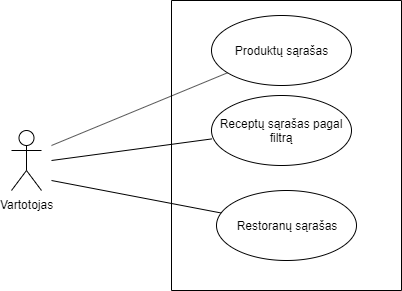
\includegraphics[scale=0.5]{/img/UseCase}
\begin{figure}[H]
    \centering
 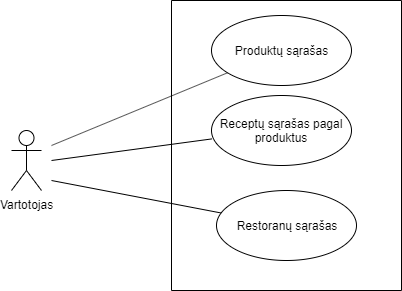
\includegraphics[scale=0.6]{img/uc}
    \caption{Sistemos naudojimo atvejų diagrama}   % Antraštė įterpiama po paveikslėlio
    \label{img:mlp}
\end{figure}
\bigskip
%\graphicspath{ {C:\Users\Max\Downloads\course_work_template_vu_mif_cs1-master\course_work_template_vu_mif_cs1-master\img\UseCase.pdf} }
1 pav.diagramoje pateiktos visos naudotojos galimybės. Naudotojas gali gauti receptų sąrašą, bet gauti receptai priklausys tik nuo prieš tai pasirinktų produktų.

\subsection{Vartotojo vykdomos  užduotys}
\subsubsection{Vartotojo užduočių dekompozicija}
\begin{figure}[H]
    \centering
 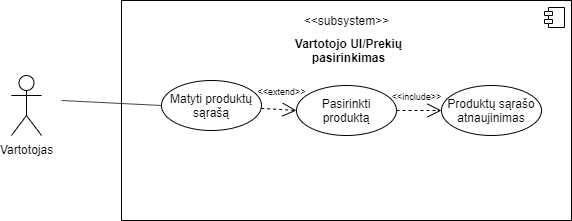
\includegraphics[scale=0.6]{img/decProd}
    \caption{Produktų išrinkimo užduočių diagrama}   % Antraštė įterpiama po paveikslėlio
    \label{img:mlp}
\end{figure}
\bigskip
2  pav. diagramoje pavaizduotos vartotojo užduotys siekiant pasirinkti prekes. Naudotojas mūsų tinkle turės galimybę pasirinkti produktus iš tam tikro sąrašo. Produktai bus išsaugoti duombazėje. 
\bigskip
\begin{figure}[H]
    \centering
 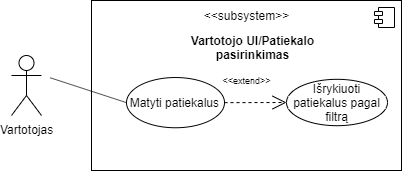
\includegraphics[scale=0.6]{img/decPat}
    \caption{Patiekalų išrinkimo užduočių diagrama}   % Antraštė įterpiama po paveikslėlio
    \label{img:mlp}
\end{figure}
\bigskip
Tuo tarpu 3 pav. pavaizduoti žingsniai norint gauti patiekalus. Patiekalai bus sudaromi iš įvairių produktų, kuriuos galėsim pasirinkti produktų skiltelėje.
\bigskip
\begin{figure}[H]
    \centering
 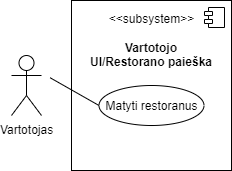
\includegraphics[scale=0.6]{img/decRest}
    \caption{Restoranų sąrašo pateikimo užduočių diagrama}   % Antraštė įterpiama po paveikslėlio
    \label{img:mlp}
\end{figure}
\bigskip
4 pav. pristatoma papildoma funkcija - restoranų sąrašo pateikimas. 


\subsubsection{Produktų išrinkimo įgyvendinimas}

\begin{figure}[H]
    \centering
 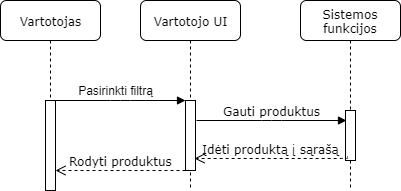
\includegraphics[scale=0.6]{img/seqProd}
    \caption{Produktų išrinkimo užduoties realizacija}   % Antraštė įterpiama po paveikslėlio
    \label{img:mlp}
\end{figure}
\bigskip
Vartotojas pasirenka produktus iš sąrašo. Paspaudus mygtuką, pasirinkti produktai išsaugomi naršymo sesijoje.

\subsubsection{Patiekalų išrinkimo įgyvendinimas}

\begin{figure}[H]
    \centering
 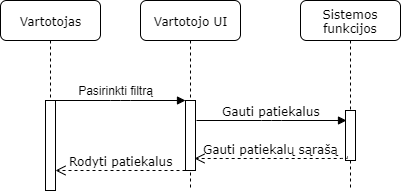
\includegraphics[scale=0.6]{img/seqPat}
    \caption{Patiekalų išrinkimo užduoties realizacija}   % Antraštė įterpiama po paveikslėlio
    \label{img:mlp}
\end{figure}
\bigskip
Patiekalų skiltelėje naudotojui bus pristatytas patiekalų sąrašas. Maistas, kurį bus galima sudaryti iš pasirinktų produktų bus žaliam fone, likusieji geltonam. Geltonam fone atsidurs tie patiekalai, kurių pagaminimui trūksta 2 patiekalų. Taip pat, kiekvienas valgis savo sudėtyje turės kalorijų skaičių ir kainą (parašyta pilna bei likusiųjų produktų kaina). Patiekalus bus galima surykiuoti pagal kainą ir kalorijas.



\subsubsection{Restoranų sąrašo pristatymo įgyvendinimas}

\begin{figure}[H]
    \centering
 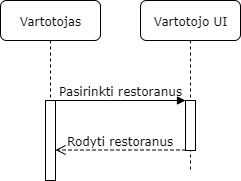
\includegraphics[scale=0.6]{img/seqRest}
    \caption{Restoranų sąrašo pristatymo užduoties realizacija}   % Antraštė įterpiama po paveikslėlio
    \label{img:mlp}
\end{figure}
\bigskip
Vartotojui pasirinkus mygtuką "Rodyti restoranus", atsiveria puslapis, kur pristatomi restoranai. Pasirinkus restoraną vartotojo naršyklėje atsidaro naujas skirtukas, kuriame rodomas restorano lokalizacija Google Maps puslapyje.

%Citavimo pavyzdžiai: cituojamas vienas šaltinis \cite{PvzStraipsnLt}; cituojami
%keli šaltiniai \cite{PvzStraipsnEn, PvzKonfLt, PvzKonfEn, PvzKnygLt, PvzKnygEn,
%PvzElPubLt, PvzElPubEn, PvzMagistrLt, PvzPhdEn}.


\section{Struktūrinis programų sistemos modelis}
\begin{figure}[H]
    \centering
 \includegraphics[scale=0.5]{img/ClassD}
    \caption{UML klasės diagrama}   % Antraštė įterpiama po paveikslėlio
    \label{img:mlp}
\end{figure}
\bigskip
Paveikslėlyje matomos visos panaudotos klasės ir vienas interfeisas HasImage. Restaurant, Product, Recipe yra pagrindinės,
 su kurių objektais naudotojas tiesiogiai sąveikaus GUI pagalba. Klasė Commands yra abstrakti klasė, kurios statiniais 
metodais paremtas sistemos veikimas. Ši klasė atsakinga už duomenų gavimą, pasirinktų produktų įsidemėjimą, 
receptų pagal pasirinktus produktus atrinkimą. Klasė receptus atrenka naudodamasi dar dviem papildomomis klasėmis: 
SortBy ir RecipeMatching. RecipeMatching klasės laukai nurodo, kiek kokiais kriterijais naudotojui trūksta iki 
recepto reikalavimų įgyvendinimo. SortBy klasės konstruktoriuje nurodama, iš statinio lauko "options" norimas rūšiavimo raktas,
 bei didėjimo ar mažėjimo tvarka (ASC ar DESC) turėtų būti pateikti receptai.
\section{Dinaminis programų sistemos modelis}

\begin{figure}[H]
    \centering
 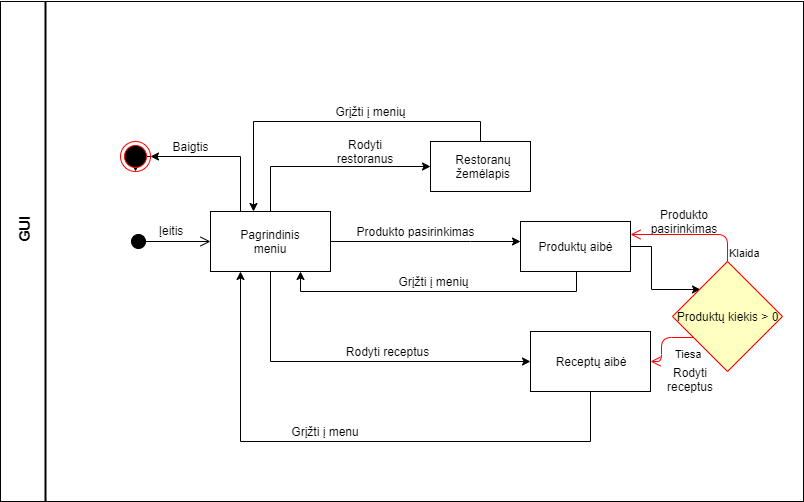
\includegraphics[scale=0.5]{img/dynamicDiagram}
    \caption{Vartotojo interfeiso būsenų diagrama}   % Antraštė įterpiama po paveikslėlio
    \label{img:mlp}
\end{figure}
\bigskip
9 pav. diagramoje pavaizduotos visos programos būsenos. Pradinė būsena - "Pagrindinis meniu", kuris bus "tarpininku" tarp kitų būsenų. 


\section{Programų sistemos komponentai}
Norint kuo tiksliau aprašyti programų sistemos loginę struktūrą - sluoksnius, posistemių hierarchiją bei fizinę struktūrą naudojami nulinis bei pirmas lygmuo.
\subsection{Nulinis lygmuo}
\begin{figure}[H]
    \centering
 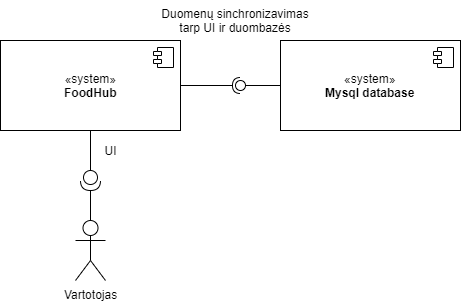
\includegraphics[scale=0.6]{img/progKomp}
    \caption{Komponentų diagrama - nulinis lygmuo}   % Antraštė įterpiama po paveikslėlio
    \label{img:mlp}
\end{figure}
\bigskip
Nulinis lygmuo pristato bendrą komponentų vaizdą. Jį sudaro 2 komponentai:
\begin{itemize}

\item {FoodHub - kuriame yra visa svarbiausia sistemos dalis}
\item {Mysql database - sistemos duomenų bazė}
\end{itemize}

\subsection{Pirmas lygmuo}
\begin{figure}[H]
    \centering
 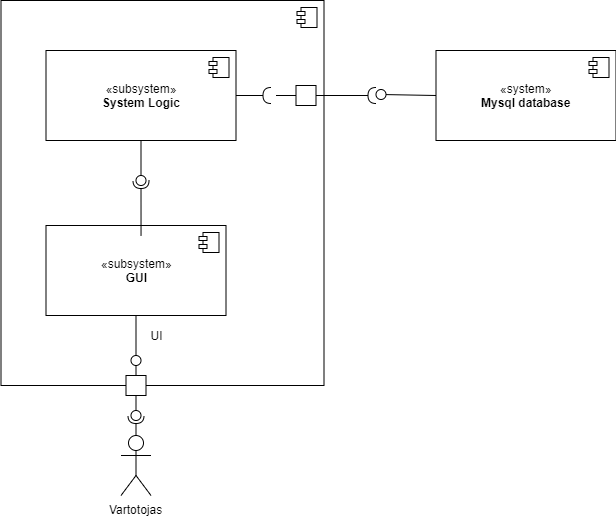
\includegraphics[scale=0.6]{img/DiagKompOne}
    \caption{Komponentų diagrama - pirmas lygmuo}   % Antraštė įterpiama po paveikslėlio
    \label{img:mlp}
\end{figure}
\bigskip
Pirmas lygmuo pristato labiau konkretų vaizdą. FoodHub komponentas buvo išskaidytas į smulkesnes dalis: "GUI" ir "System Logic". "System Logic" komponentas yra tarpininku tarp "GUI" ir duomenų bazės. Jame yra sistemos funkcijų realizacija.


\section{Komponentų išskirstymas tinkle}
\begin{figure}[H]
    \centering
 \includegraphics[scale=0.6]{img/foodkomp}
    \caption{Programų sistemos komponentų išdėstymas tinkle}   % Antraštė įterpiama po paveikslėlio
    \label{img:mlp}
\end{figure}
\bigskip
Numatomas išdėstymas tinkle:
%Numatomas išdėstymas tinkle:

\begin{small}
%\vspace{-5mm}
\begin{itemize}[noitemsep,topsep=0pt]
\setlength\itemsep{0em}
\item {Nuotoliniame serveryje duomenų bazė saugojanti duomenis}
\item {Internetinė svetainė patalpinta serveryje}
\item {Vartotojas pasiekia serverį su internetine naršyklę}
\end{itemize}

\end{small}

\section{Prototipo aprašymas}

\subsection{Pradinis prototipas. Jo aprašymas}
Pasikrovus puslapiui, pirmas matomas langas yra pasirinkimo langas, naudotojas turi pasirinkti, ar jis nori įvesti produktus kuriuos turi, ar iš karto gauti receptų sąrašą, ar tiesiog nori gauti restoranų sąrašą.

\begin{figure}[H]
    \centering
 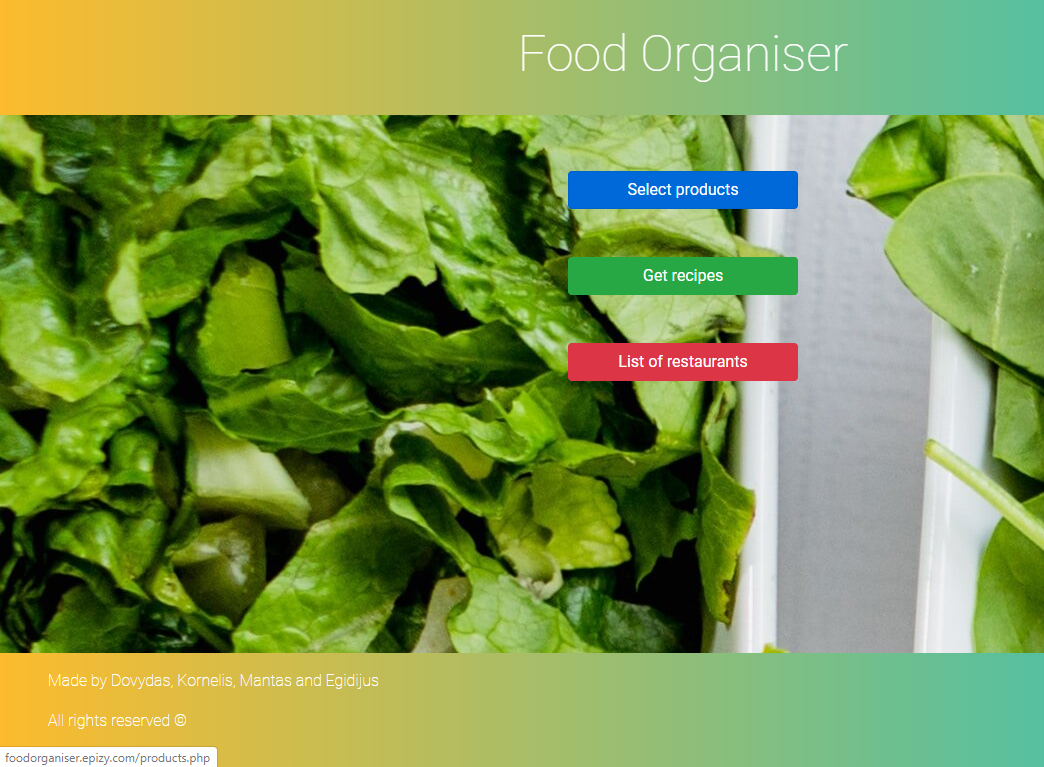
\includegraphics[scale=0.5]{img/startWindow}
    \caption{Pradinis sistemos langas}   % Antraštė įterpiama po paveikslėlio
    \label{img:mlp}
\end{figure}
\bigskip

Pasirinkus "Get recipes" naudotojui parodomas produktų sąrašas iš kurio jis gali pasirinkti kuriuos produktus jis turi. Parinkus "Select products" vartotojas gali patvirtinti pasirinkimą, tuomet jis perkeliamas į receptų sąrašo langą, kuriame rodomi tinkamiausi receptai. Paspaudus "List of restaurants" naudotojas gali pamatyti artimiausius restoranus Google Maps žemėlapyje.

\begin{figure}[H]
    \centering
 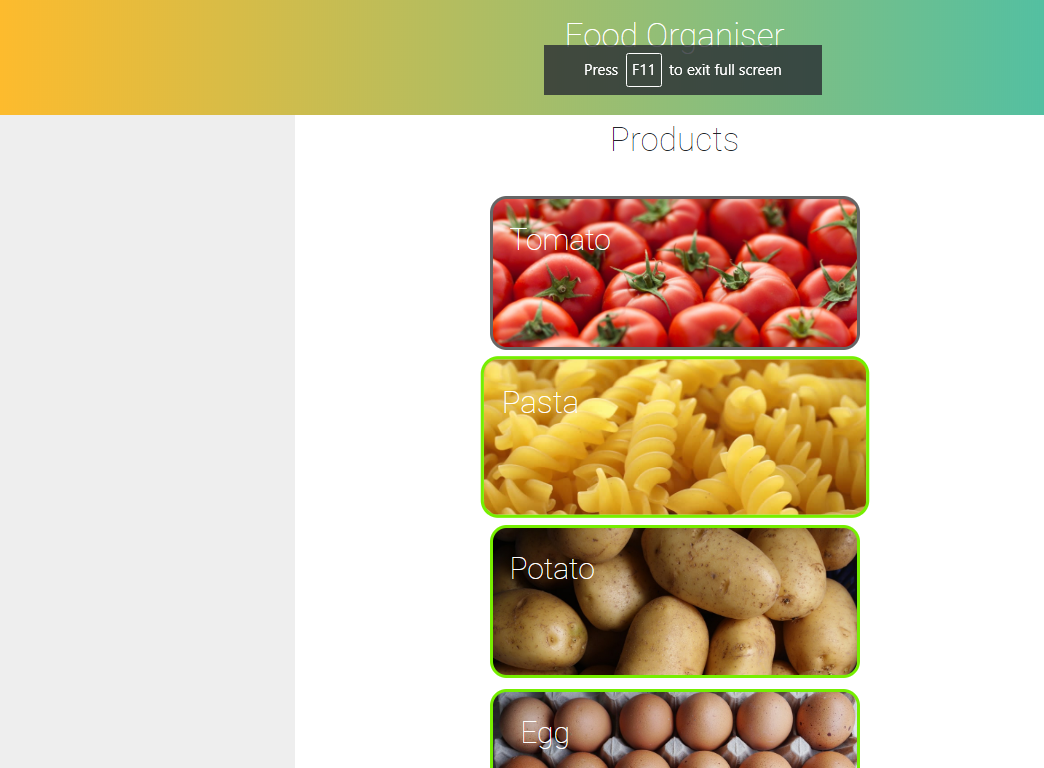
\includegraphics[scale=0.5]{img/selectProducts}
    \caption{Produktų pasirinkimo langas}   % Antraštė įterpiama po paveikslėlio
    \label{img:mlp}
\end{figure}
\bigskip

Pasirinkus "Select product" naudotojui parodomas produktų sąrašas iš kurio jis gali pasirinkti kuriuos produktus jis turi. Parinkus produktus žmogus gali patvirtinti pasirinkimą, tuomet jis perkeliamas  į receptų sąrašo langą, kuriame rodomi tinkamiausi receptai.

\begin{figure}[H]
    \centering
 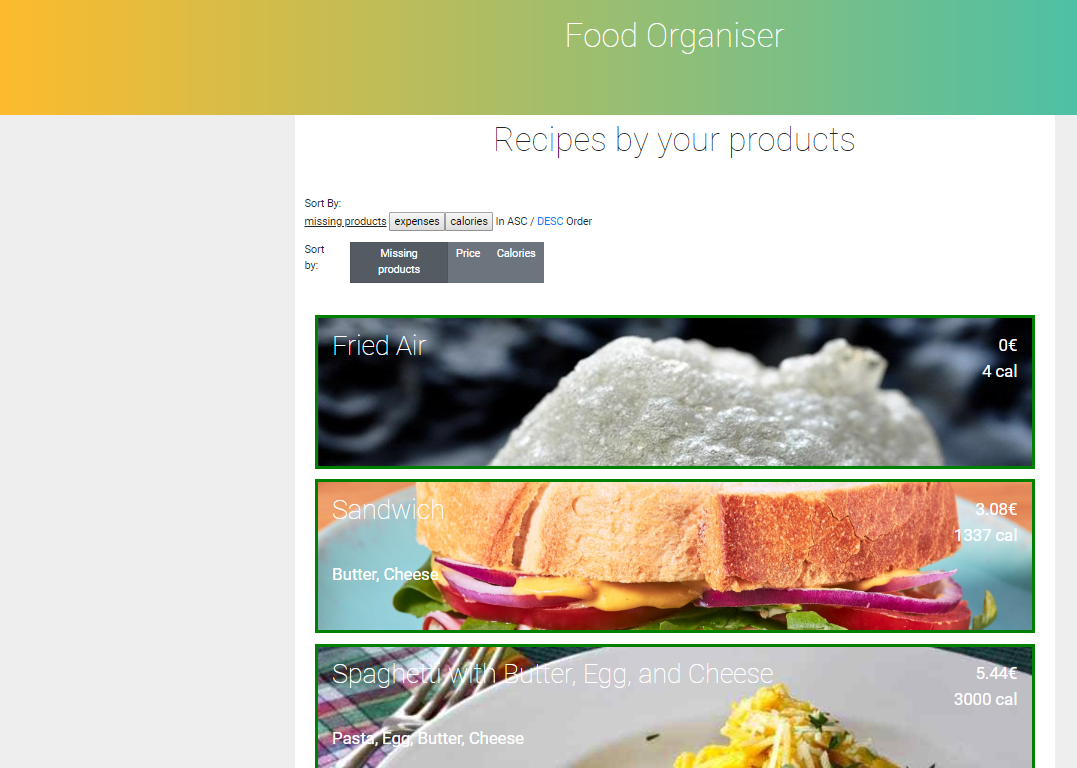
\includegraphics[scale=0.5]{img/recipes}
    \caption{Patiekalų sąrašas}   % Antraštė įterpiama po paveikslėlio
    \label{img:mlp}
\end{figure}
\bigskip

Patekus į "Select recipes" žmogus mato jam labiausia tinkančius receptus. Prie receptų parašyta jų kaina, kalorijų kiekis ir produktų sąrašas.

\begin{figure}[H]
    \centering
 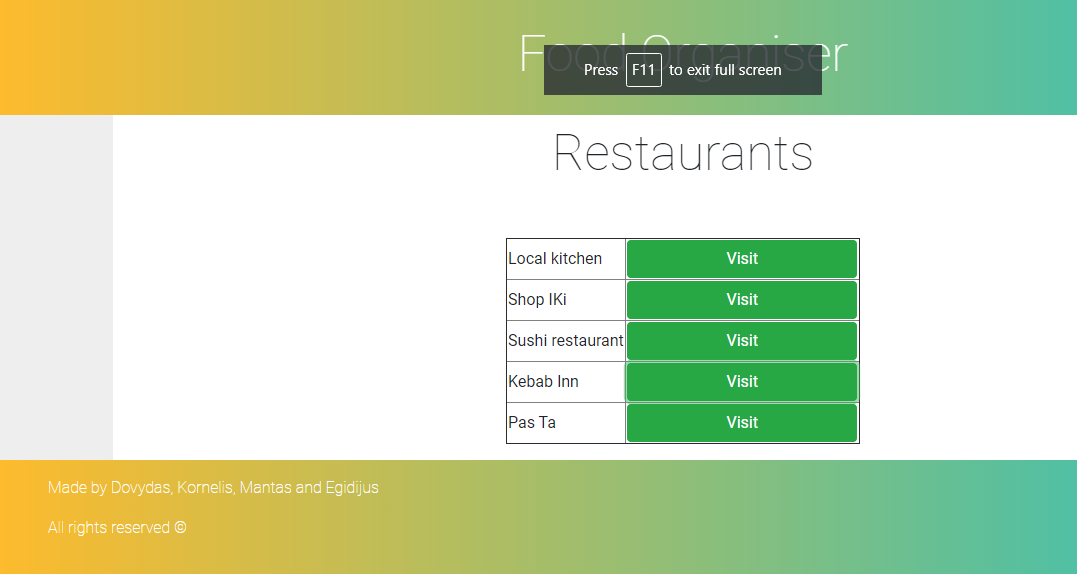
\includegraphics[scale=0.5]{img/restaurants}
    \caption{Artimiausių restoranų sąrašas}   % Antraštė įterpiama po paveikslėlio
    \label{img:mlp}
\end{figure}
\bigskip

Pasirinkus "Select restaurant" jam parodomas restoranų sąrašas. Pasirinkus kurį nors restorano pavadinimą jam parodoma pasirinkto restorano vietovė. 

\sectionnonum{Išvados}
Darbe įgyvendinti iškelti uždaviniai pasinaudojus 4+1 architektūros pjūvių modelį:
\begin{small}
%\vspace{-5mm}
\begin{itemize}[noitemsep,topsep=0pt]
\setlength\itemsep{0em}
\item {Aprašyti sistemos vykdymo scenarijai}
\item {Apibrėžtos klasės bei ryšiai tarp jų}
\item{Pristatyta programų sistemos elgsena jos vykdymo metu}
\item {Nurodyti sistemos komponentai bei jų išskirstymas tinkle}
\item{Atliktas sistemos prototipas}
\end{itemize}

\end{small}
\bigskip
Šios užduoties vykdymo metu, architektūros pjūvių modeliai ir pats prototipas buvo keletą kartų tobulinami, kad abu atspindėtų siekiamą tikslą. Galiausiai galima teigti, jog darbo idėja buvo įgyvendinta. Sukurta internetinė svetainė, kuri savo funkcionalumu atvaizduoja FoodHub sistemą.

\printbibliography[heading=bibintoc] % Literatūros šaltiniai aprašomi
% bibliografija.bib faile. Šaltinių sąraše nurodoma panaudota literatūra,
% kitokie šaltiniai. Abėcėlės tvarka išdėstoma tik darbe panaudotų (cituotų,
% perfrazuotų ar bent paminėtų) mokslo leidinių, kitokių publikacijų
% bibliografiniai aprašai (šiuo punktu pasirūpina LaTeX). Aprašai pateikiami
% netransliteruoti.

\appendix  % Priedai
% Prieduose gali būti pateikiama pagalbinė, ypač darbo autoriaus savarankiškai
% parengta, medžiaga. Savarankiški priedai gali būti pateikiami kompiuterio
% diskelyje ar kompaktiniame diske. Priedai taip pat vadinami ir numeruojami.
% Tekstas su priedais siejamas nuorodomis (pvz.: \ref{img:mlp}).



\end{document}
